%\pagestyle{fancy}
\chapter{Experimental Setup}
\label{ch:ExperimentalSetup}

\section{Sensors}
\subsection{IMU}
\begin{figure}[htb]
	\centering
	%todo Add 3d coordinate system and trim image
	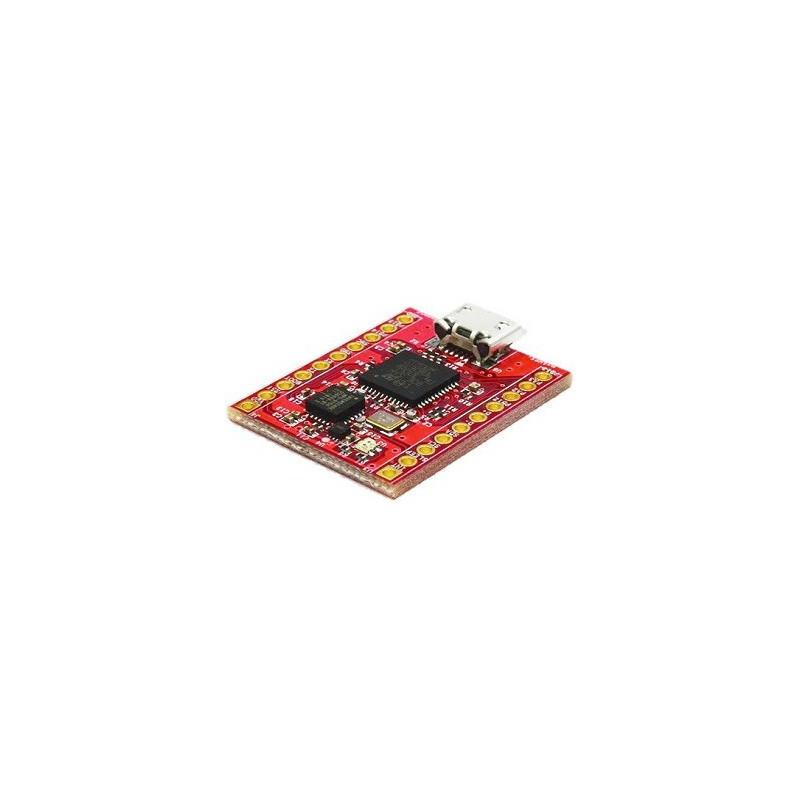
\includegraphics[clip, trim={8cm 8cm 8cm 8cm}, width=0.3\linewidth]{IMU.jpg}
	% 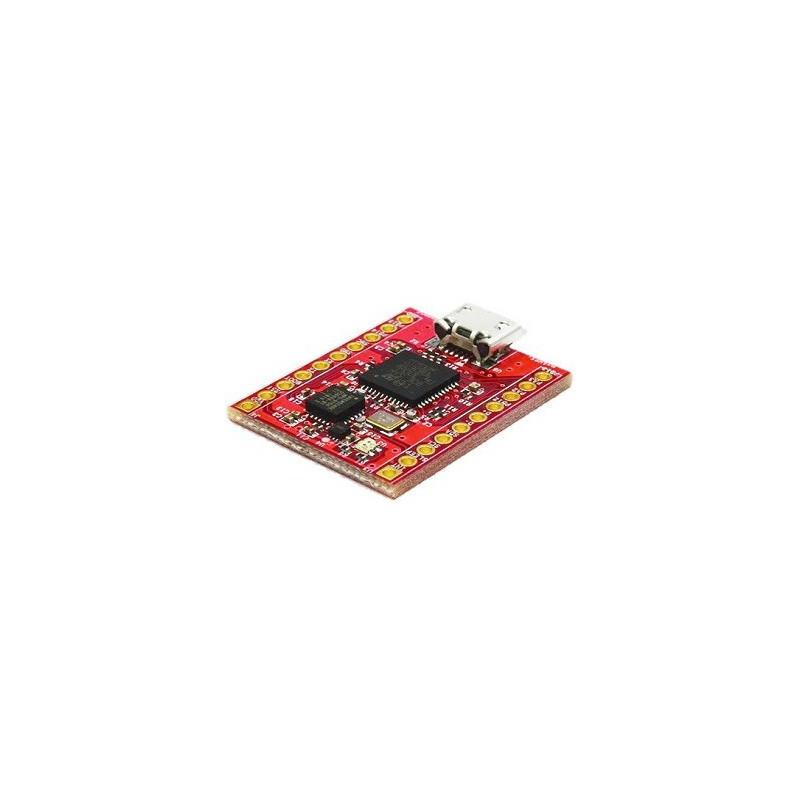
\includegraphics[width=0.7\linewidth]{IMU.jpg}
	\caption[myAHRS+ IMU]{myAHRS+ IMU this is the long caption which does not show up in list of figures \itodo{higher resolution + trim; add coordinate system}}
	\label{fig:imu}
\end{figure}
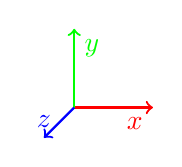
\begin{tikzpicture}
    \coordinate (O) at (0,0,0);
    \draw[thick,->, red] (0,0,0) -- (1,0,0) node[anchor=north east]{$x$};
    \draw[thick,->, green] (0,0,0) -- (0,1,0) node[anchor=north west]{$y$};
    \draw[thick,->, blue] (0,0,0) -- (0,0,1) node[anchor=south]{$z$};
\end{tikzpicture}

For the experiments the myAHRS+, a low cost high performance \gls{ahrs} will be used.
An AHRS contains an IMU and outputs the raw data but also has an integrated Kalman filter which calculates the pose in form of quaternion or euler angles.
It offers an micro-USB interface and runs with up to \SI{100}{\Hz}.
It can capture a change of $\pm$2000 dps (degrees per second), $\pm$16 $g$ and $\pm$\SI{1200}{\micro\tesla}.
During the experiment only a fraction of this range is expected to be reached, hence the sensor seems suitable.
Besides the hardware the unit already has an Extended Kalman Filter (EKF) on board.
The EKF fuses the measurements of the three sensors and estimates a quaternion (and sth else?) from it.
But this will not be used.

\subsection{Lidar}
Two different LiDARs will be used during the experiment.
The RS-Bpearl and the Velodyne UltraPuck.
The most relevant specifications of the two LiDARs can be seen in table \ref{tab:lidar_datasheets}.
Both are mechanical LiDARs and have the same number of laser channels, but the Velodyne has a significant better vertical resolution, due to the smaller vertical FOV.

\begin{table}[ht]
	\centering
	% todo: Manual citation prop wrong
	\caption{Comparison of the two used LiDARs \cite{RoboSense2020}\cite{Rev}}
	\label{tab:lidar_datasheets}
	\begin{tabular}[t]{lcc}
	\toprule
	&\textbf{RS-Bpearl} & \textbf{Velodyne Ultra Puck}\\
	\midrule
	Channels 				& 32 							& 32\\
	Range 					& \SI{100}{\metre}				& \SI{200}{\metre}\\
	Range accuracy			& $\pm\SI{3}{\centi\metre}$		& $\pm\SI{3}{\centi\metre}$\\
	Horizontal FOV		 	& \SI{360}{\degree}				& \SI{360}{\degree}\\
	Vertical FOV 			& \SI{90}{\degree}				& \SI{40}{\degree}\\
	Horizontal resolution	& \SIrange{0.2}{0.4}{\degree} 	& \SIrange{0.1}{0.4}{\degree}\\
	Vertical resolution		& \SI{2.81}{\degree} 			& \SI{0.33}{\degree}\\
	Frame rate 				& \SIrange{10}{20}{\hertz}		& \SIrange{5}{20}{\hertz}\\
	Laser wavelength 		& \SI{905}{\nano\metre} 		& \SI{903}{\nano\metre}\\
	% \midrule
	Points per second 		& 576,000						& 600,000		\\
	\bottomrule
	\end{tabular}
	\end{table}%

\missingfigure{Picture of robosense or/and velodyne}

\subsection{Placement}
\begin{figure}[htpb]
    % Distance for measurement line
    \def\dd{.4cm}
	\centering
	\begin{tikzpicture}[scale=1, spy using outlines={red, circle, magnification=3, size=4cm, connect spies}]
		% RAMP
        % Define/Calc ramp parameters
        % Ramp length
        \def\rl{5};
        % Ramp angle [deg]
        \def\ra{15};
        % Ramp height
        \def\rh{{tan(\ra)*\rl}};

		% Define the points
		\coordinate (A) at (0,0);
		\coordinate (B) at ($(A) + (\rl,0)$);
		\coordinate (C) at ($(B) + (0,\rh)$);
        % Draw and fill ramp
		\filldraw[draw=black, fill=lightgray!25] (A) -- (B) -- (C) -- cycle;
        % Draw angle
        \path (A) -- (B)
		pic[draw, ->, angle radius=40pt,
		angle eccentricity=0.75, "$\alpha$"]{angle=B--A--C};
		% Ground and helpers
		\coordinate (D) at ($(A) + (-10,0)$);
		\draw [thick] (D) -- (A) -- (C);

        % CAR
        \begin{scope}[scale=0.7]
            % Car height
            \def\ch{2}
            % Car length
            \def\cl{5}
            % Car body height
            \def\bh{\ch*0.65}
            % Roof length
            \def\rl{\cl*0.6}
            % Roof height
            \def\rh{\ch*0.35}
            % Car tilt angle
            \def\ct{6}
			% Anchor point is southwest
			\coordinate (b) at ($(D) + (0,0.5)$);
			% Offset to roof and wheels
			\coordinate (r) at ($(b) +(\cl*0.17,\ch*0.65)$);
			\coordinate (w) at ($(b) + (\cl*0.25,0)$);

			% Body
			\draw[black, fill=black!17, rounded corners=1.2ex, very thick]
			(b) -- ++(0,\bh) -- ++(\cl*1/5,0) --  ++(\cl*3/5,0) -- ++(\cl*1/5,-\bh*0.25)
			-- ++(0, -\bh*0.75) -- (b) -- cycle;
			% Roof
			\draw[very thick, rounded corners=0.5ex, fill=black!20!blue!20!white,thick]
			(r) -- ++(0.2*\rl,\rh) -- ++(0.5*\rl,0) -- ++(0.3*\rl,-\rh) -- (r);
			% \draw[thick] ($(r) + (\cl*0.5,\bh)$) -- ++(0,\rh);
			\draw[thick] (r)++(\rl*0.6,0) -- ++(0,\rh);

			% Wheels
			\draw[draw=black,fill=gray!50,thick] (w) circle (.5);
			\draw[draw=black,fill=gray!50,thick] (w) ++(\cl*0.55,0) circle (.5);
			% Inner wheels
			\draw[draw=black,fill=gray!80,semithick] (w) circle (.35);
			\draw[draw=black,fill=gray!80,semithick] (w) ++(\cl*0.55,0) circle (.35);

			% Lidar
			\draw[black, fill=red!50] ($(r) + (\cl*0.40,\rh)$) coordinate (le) arc(-10:180:0.4) --cycle;

			% Car middle point
			\coordinate (m) at (\cl*0.5, \bh*0.5);
			% Lidar middle point
			\coordinate (lm) at ($(le) + (-0.39,0.2)$);
            \filldraw[red] (lm) circle(.1);

			% Laser lines
			\draw[->,color=red,decorate,decoration={snake,amplitude=.2mm,segment length=1mm,post length=1mm}] (lm) -- (A);
			\draw[->,color=red,decorate,decoration={snake,amplitude=.2mm,segment length=1mm,post length=1mm}] (lm) -- ($(A)!0.5!(C)$);
			\path (lm) -- (A)
			pic[draw, ->, angle radius=70pt, angle eccentricity=0.9,
			"$\beta$"]{angle=A--lm--B};
        \end{scope}

        % \dimline[extension start length=-\dd, extension end length=-\dd] {($(D)+(0,-\dd)$)}{($(A)+(0,-\dd)$)}{$d$};
		\dimline[extension start length=\dd, extension end length=\dd] {($(A)+(0,-\dd)$)}{($(A)!0.4!(D)+(0,-\dd)$)}{$d$};
		\dimline[extension start length=\dd, extension end length=\dd+1.9cm] {($(lm)+(0,\dd)$)}{($(lm -| A)+(0,\dd)$)}{$d$};
        \dimline[extension start length=-\dd, extension end length=-\dd] {($(A)+(0,-\dd)$)}{($(B)+(0,-\dd)$)}{$l$};
        \dimline[extension start length=-\dd, extension end length=-\dd] {($(B)+(\dd,0)$)}{($(C)+(\dd,0)$)}{$h_\mathrm{r}$};
        \dimline[extension start length=\dd, extension end length=\dd+1.7cm] {($(D)+(-\dd,0)$)}{($(lm -| D)+(-\dd,0)$)}{$h$};
        % \draw (D) -- (lm -| D);
        % \dimline[extension start length=-\dd, extension end length=-\dd] {($(lm)+(\dd,0)$)}{($(C)+(\dd,0)$)}{$h_2$};
        % \dimline[extension start length=\dd, extension end length=\dd] {($(A)+(0,\dd)$)}{($(C)+(0,\dd)$)}{$d$};
		% \spy on ($(lm)!.05!(A)$) in node at (3,4);
		\spy on (lm) in node at (3,4);


	\end{tikzpicture}
	\caption{Mounting of the LiDAR}
\end{figure}

The LiDAR will be placed on top of the car, to get a greater FOV.
The pitch angle at which the LiDAR will be mounted should be chosen so that the number of points in the area at the beginning of the ramp are maximized.
This allows for an easier detection of planes with different inclination angles.
The coordinates at which the lasers hit the ground and ramp depend on the height of the LiDAR $ h_\mathrm{L} $, the distance to the ramp $d$, the angle of the ramp $\alpha$, the pitch angle $\gamma$ at which the LiDAR is mounted and finally on the vertical resolution and FOV of the LiDAR. The coordinates can be calculated in the following way.\\
Up to $d$ the points will hit the ground, the
\itodo{Make a good sketch again with labels etc and check if its easy understandable, only then continue in tikz and latex}
\begin{equation}
	\alpha
\end{equation}

\[ c = h - \frac{z}{\tan \alpha} \]

\subsection{Odometry}
\todoin{
  \begin{itemize}
	\item What is it and where used
	\item very short how does it work
	\item maybe calculation of velocity from ticks here
  \end{itemize}}

\section{Car}
\missingfigure{Picture of eGolf}

\section{Garage}
\missingfigure{Picture of ramps or figure of ramps showing angles}


%\subsubsection{Mechanical}
%One of the earliest realization of a gyroscope and consists of a platform and three (or two?!) gimbals.
%\subsection{Optical}
%More precise but also more expensive are optical gyroscopes. It uses the signac effect, which says that it takes longer to travel a circular path with the direction of rotation, than it does against. A coil of optical fiber with multiple loops is setup and a laser beam is sent in both directions and the interference of the two beams is measured. Due to the high speed of light the path has to be long enough (>\SI{100}{\metre}), to allow for a measurable result.